\subsection{Detector Nonlinearity}
\label{det_nonlinearity}

\paragraph{Description:}
For transition-edge sensors (TESs), we expect inherent detector nonlinearity for incoming microwave power violating the ``small-signal'' limit. This limit is not defined absolutely in temperature fluctuations or microwave power units, but must be compared to the ability of the detector to ``linearize'' its response through a large loop gain $L$ (a function of detector parameters  like the logarithmic derivative $dlnR/dlnT = \alpha$ and the Joule power $ P_{\mbox{\scriptsize b}}$ on the bolometer) and negative feedback (provided by that same Joule power when the detector is stiffly voltage-biased). If a large enough input signal, over whatever timescale, can swamp the ability of the detector to maintain linearity, we are no longer able to assume a single well-calibrated gain for that detector to any important physical unit such as incoming microwave power or on-sky temperature fluctuations.

There have been studies of TES nonlinear response excited by large transients or sinusoidal input signals \cite{Rostem} \textbf{add reference to syst.bib file}. This detailed model based on tracking time variation of TES parameters like $\alpha$ should be compared to the effective description which was found to be useful for data featuring a HWP in the POLARBEAR-1 experiment \cite{PB1_WHWP}. This result is further discussed in Section \ref{hwp_non_linearity}. A generic description of nonlinearity is Eq. 2.9 in that paper, where, for a detector timestream $d(t)$:

\begin{equation}
d'(t) = [ 1 + g_1 d(t) ] d(t - \tau_1 d(t)).
\label{nonlinearity}
\end{equation}

The nonlinearity parameters $g_1$ and $\tau_1$, when studied assuming perfectly-stiff voltage feedback (or voltage fluctuations $\delta V = 0$), reduce to ratios of linear model parameters multiplied by a quantity $C$ which contains all second-order derivatives of the TES resistance $R(T,I)$. In the particular case of the paper, the form of these parameters is derived and compared to data to determine the value of $C$. However, this derivation is for the specific case of incoming power at two distinct frequencies (where nonlinearity will couple the two) and sending the frequency of the lower to 0. Thus $g_1$ and $\tau_1$ are functions of some modulation frequency, which is not relevant for experiments without HWPs.

Schematically, a complete result is the following, where, after attempting to calibrate measured current fluctuations using linear theory, we find:

\begin{equation}
\delta P_{\mbox{\scriptsize meas}} (t) = \delta P_{\mbox{\scriptsize opt}} (t) + \delta^2 I (t) * \delta P_{\mbox{\scriptsize opt}}/dI.
\label{nonlinear_sum}
\end{equation}
In short, the nonlinearity in general represents a complicated signal biasing our recovered measurement of the microwave power fluctuations.

\paragraph{Plan to model and/or measure:}
Using only the bare detectors, we can directly estimate $g_1$ and $\tau_1$ as a function of input signal amplitude using test tones and looking at the amplitude and phase of the second harmonic relative to the first. This would be relevant for the model of Eq. \ref{nonlinearity}, and should be compared to those measured by the POLARBEAR-1 team using their distinct method.

Modeling the possible biases induced by these parameters is being done within a complete systematics simulation framework, where the equation is used to ``reobserve'' detector timestreams which are then projected back into map space. Since the case in the presence of a HWP has been well commented upon in other sections, this simulation will specifically focus on correlated noise coupling to nonlinearity to induce uncalibrated, time-varying differential gain between polarization-pair detectors. This is a direct path for low-frequency correlated modes to enter polarization maps (Fig. \ref{QU leakage}). Given the magnitude of this effect for POLARBEAR-1 like devices, and the fact that we do not yet have full models of these effects, we rate this systematic as SRF = 5.

\begin{figure}[h!]
\centering
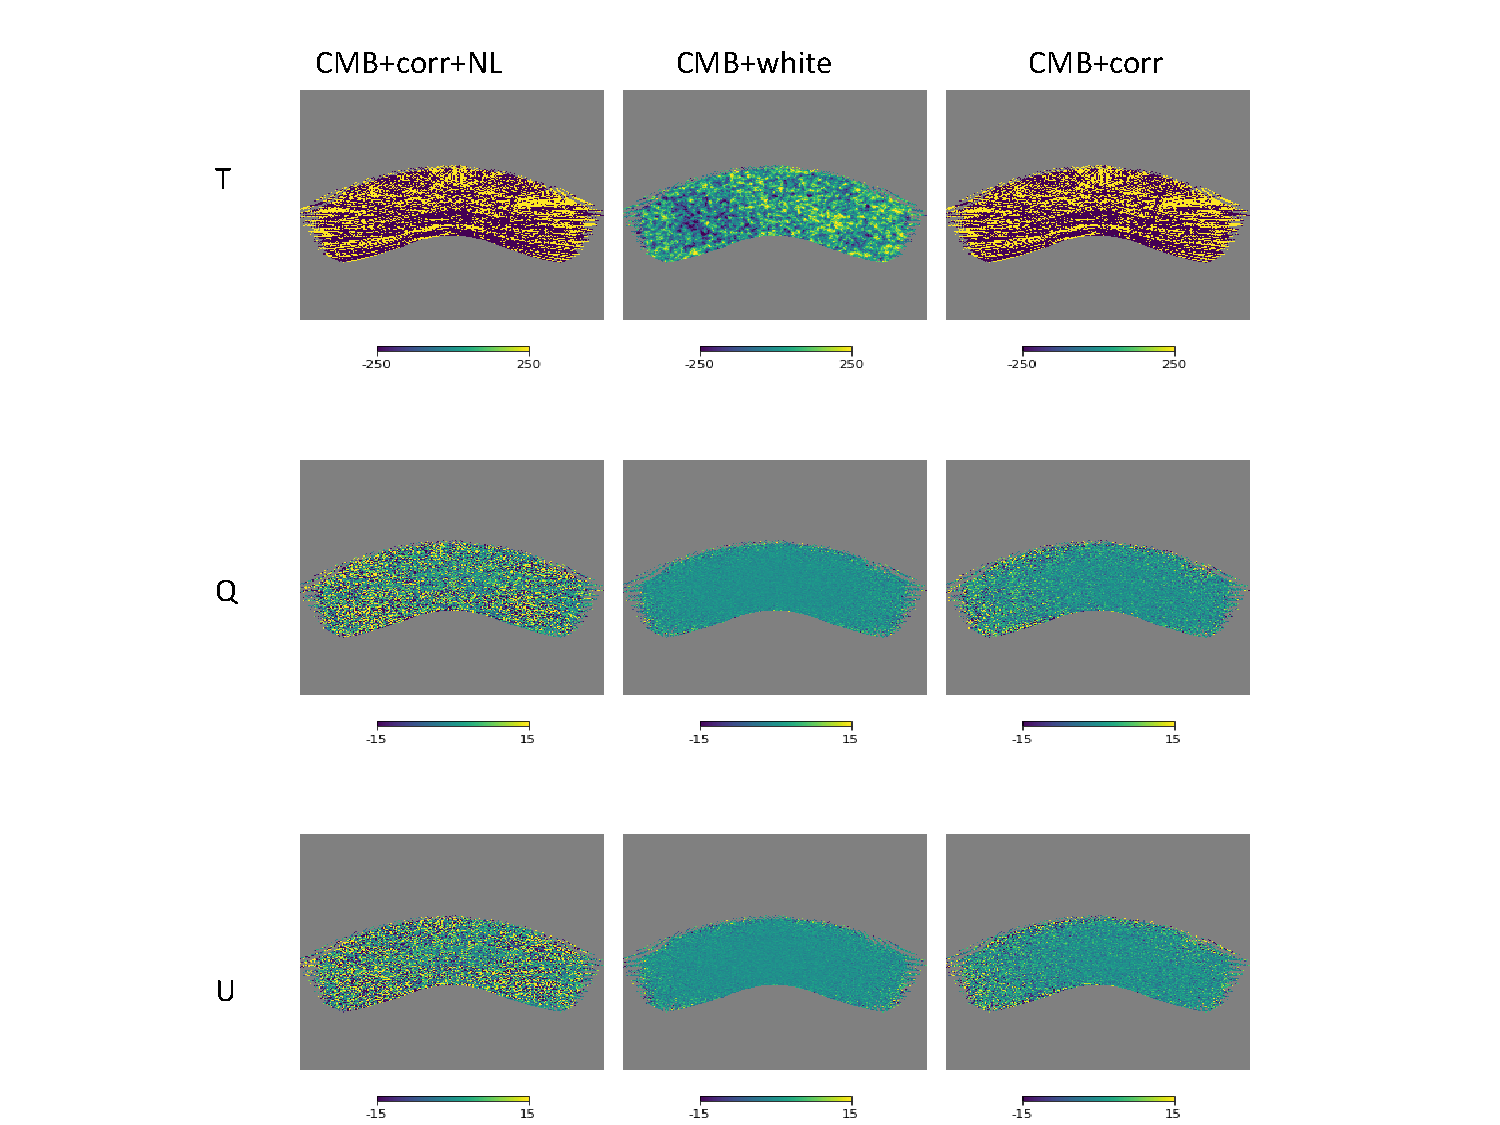
\includegraphics[width=0.85\textwidth]{figures/040218_s4cmb_corr_NL.pdf}
\caption{Pure T->P leakage maps generated with s4cmb for an example instrument and experiment. The middle column is pure CMB+white noise (minimal leakage), the right column is CMB+white+correlated noise, and the left is the same as the right but observed through the nonlinearity equation. Random draws of $g_1$ and $\tau_1$ were performed for each detector in the focal plane.}
\end{figure}

\paragraph{Uncertainty/Range:}
Current results from \cite{PB1_WHWP} quote rough estimates of $g_1 \sim$ 0.8 \%/K and $\tau_1 \sim$ 0.1 ms/K, where we assume $d(t)$ have been calibrated to CMB temperature using a conversion factor. Data for Advanced ACTPol detectors in the field with no sky loading show XX\% ratio of second-harmonic to first-harmonic amplitude.

\paragraph{Parameterization:}
We currently plan to use the simpler equation to determine what acceptable limits on $g_1$ and $\tau_1$ are demanded by science goals. When summarized in terms of TES design parameters, we can then feed these requirements back to the detector design group.